\documentclass[11pt,a4paper]{article}
\usepackage[margin=2.2cm]{geometry}
\usepackage{amsmath,amssymb}
\usepackage{graphicx}
\usepackage{booktabs}
\usepackage{tabularx}
\usepackage{array}
\usepackage{multirow}
\usepackage{float}
\usepackage{caption}
\usepackage{subcaption}
\usepackage{xcolor}
\usepackage{enumitem}
\usepackage{fancyhdr}
\usepackage[hidelinks]{hyperref}

\graphicspath{{figures/}}
\setlist{itemsep=2pt,topsep=4pt}
\captionsetup{font=small,labelfont=bf}
\newcommand{\R}{\mathbf{R}}
\newcommand{\tv}{\mathbf{t}}
\newcommand{\K}{\mathbf{K}}
\newcommand{\X}{\mathbf{X}}
\newcommand{\best}[1]{\textbf{#1}}

\setlength{\headheight}{14pt}
\pagestyle{fancy}
\fancyhf{}
\lhead{Computer Vision (CS6350)}
\rhead{Compute change in pose (3D) of a small object}
\cfoot{\thepage}

\begin{document}

% ---------------------------------------------------------------- title page
\begin{titlepage}
\centering
{\Large Indian Institute of Technology Madras\par}
\vspace{2.5cm}
{\large (TPA 12)\par}
\vspace{0.4cm}
{\LARGE\bfseries Compute change in pose (3D) of small objects\par}
\vspace{2.5cm}
{\large Course: CS6350 -- Computer Vision\par}
{\large Professor: Dr.\ Sukhendu Das\par}
\vfill
{\large Members:\par}
{\large Sai Svanik Chiramana (ME23B195)\par}
{\large Sathwik Chanduluri (ME23B238)\par}
\vspace{1.5cm}
\end{titlepage}

% ---------------------------------------------------------------- abstract
\begin{abstract}
\noindent We estimate the change in 3D pose of a small object between two RGB photographs: the
rotation $\R$, the direction of the translation $\tv$, and the reprojection error of the matched
points. The pipeline crops the images around the object, finds point correspondences with one
of eight matchers (classical SIFT, learned sparse matchers, the dense matcher LoFTR and the 3D
foundation model MASt3R), fits a homography and an essential matrix with MAGSAC++, lets
Torr's GRIC criterion choose between them, and refines the pose with Levenberg--Marquardt.
Matchers are also combined into three \emph{cascades} (\texttt{fast}, \texttt{accurate},
\texttt{confident}), the last of which uses a learned confidence model to decide when the
expensive matcher is needed. Everything runs on a laptop CPU. On 751 held-out test pairs from four
public real-image datasets (TUM RGB-D, Objectron, CO3D, MVImgNet), MASt3R reaches a mean
AUC@10 of 73.0\% with a median rotation error of 0.90$^\circ$; the \texttt{confident} cascade
reaches 64.0\% at a median of 0.7\,s per pair; SIFT alone reaches 35.8\%. For photographs with
no calibration and no annotation, an automatic front end estimates the focal length and finds
the object region, and costs only 4--5 points of AUC@10 on TUM and Objectron.
\end{abstract}

\tableofcontents
\newpage

% ================================================================ 1
\section{Problem statement}

The task (TPA-12) is to \emph{compute the change in 3D pose of a small object} from two RGB
images. Concretely, given two views $I_1, I_2$ of the same object, we must output
\begin{itemize}
  \item the \textbf{relative rotation} $\R \in SO(3)$ and the \textbf{translation} $\tv$ that map
        a 3D point from camera-1 coordinates to camera-2 coordinates,
        \begin{equation}
          \X_2 = \R\,\X_1 + \tv ,
        \end{equation}
        in the OpenCV camera convention ($x$ right, $y$ down, $z$ forward);
  \item the \textbf{reprojection error} of the matched points under the estimated pose.
\end{itemize}
If the camera is still and the object moves, $(\R,\tv)$ is the object's own motion expressed
in the camera's axes; if the object is still and the camera moves, it is the camera's motion
relative to the object. Two views fix $\tv$ only up to scale, so its \emph{direction} is
estimated; its length is recovered only when the object's size is known
(Section~\ref{sec:scale}).

What makes the problem hard:
\begin{itemize}
  \item \textbf{Small objects.} The object covers a small part of the image (a key, a coin, a
        phone), so it yields few features, while the background yields many. Matches on the
        background describe the background, not the object.
  \item \textbf{Little texture.} Phone backs, watch faces and dark wallets are smooth, shiny or
        dark, so keypoint detectors find little to match.
  \item \textbf{Near-planar objects.} Books, phones and posters are almost flat. The essential
        matrix is ill-conditioned on a plane, and a plane admits two physically valid poses.
  \item \textbf{Large viewpoint changes} of 30--60$^\circ$ change the object's appearance.
  \item \textbf{Unknown camera.} Photos handed over at a demo carry no intrinsics and no
        object annotation.
\end{itemize}

Our constraints: only public datasets of real images with ground-truth poses (no synthetic
data), CPU only, and every reported number on pairs that were never used for tuning.

% ================================================================ 2
\section{Pipeline overview}

Figure~\ref{fig:pipeline} shows the full processing chain. The \emph{core pipeline} (blue)
takes two images, the camera intrinsics $\K$ and the object's region in each image, and
produces the pose. Every benchmark number in this report comes from it. The \emph{automatic
front end} (orange) is used only for photographs about which nothing is known: it estimates the
focal length and finds the object region, then hands both to the same core pipeline.

\begin{figure}[H]
  \centering
  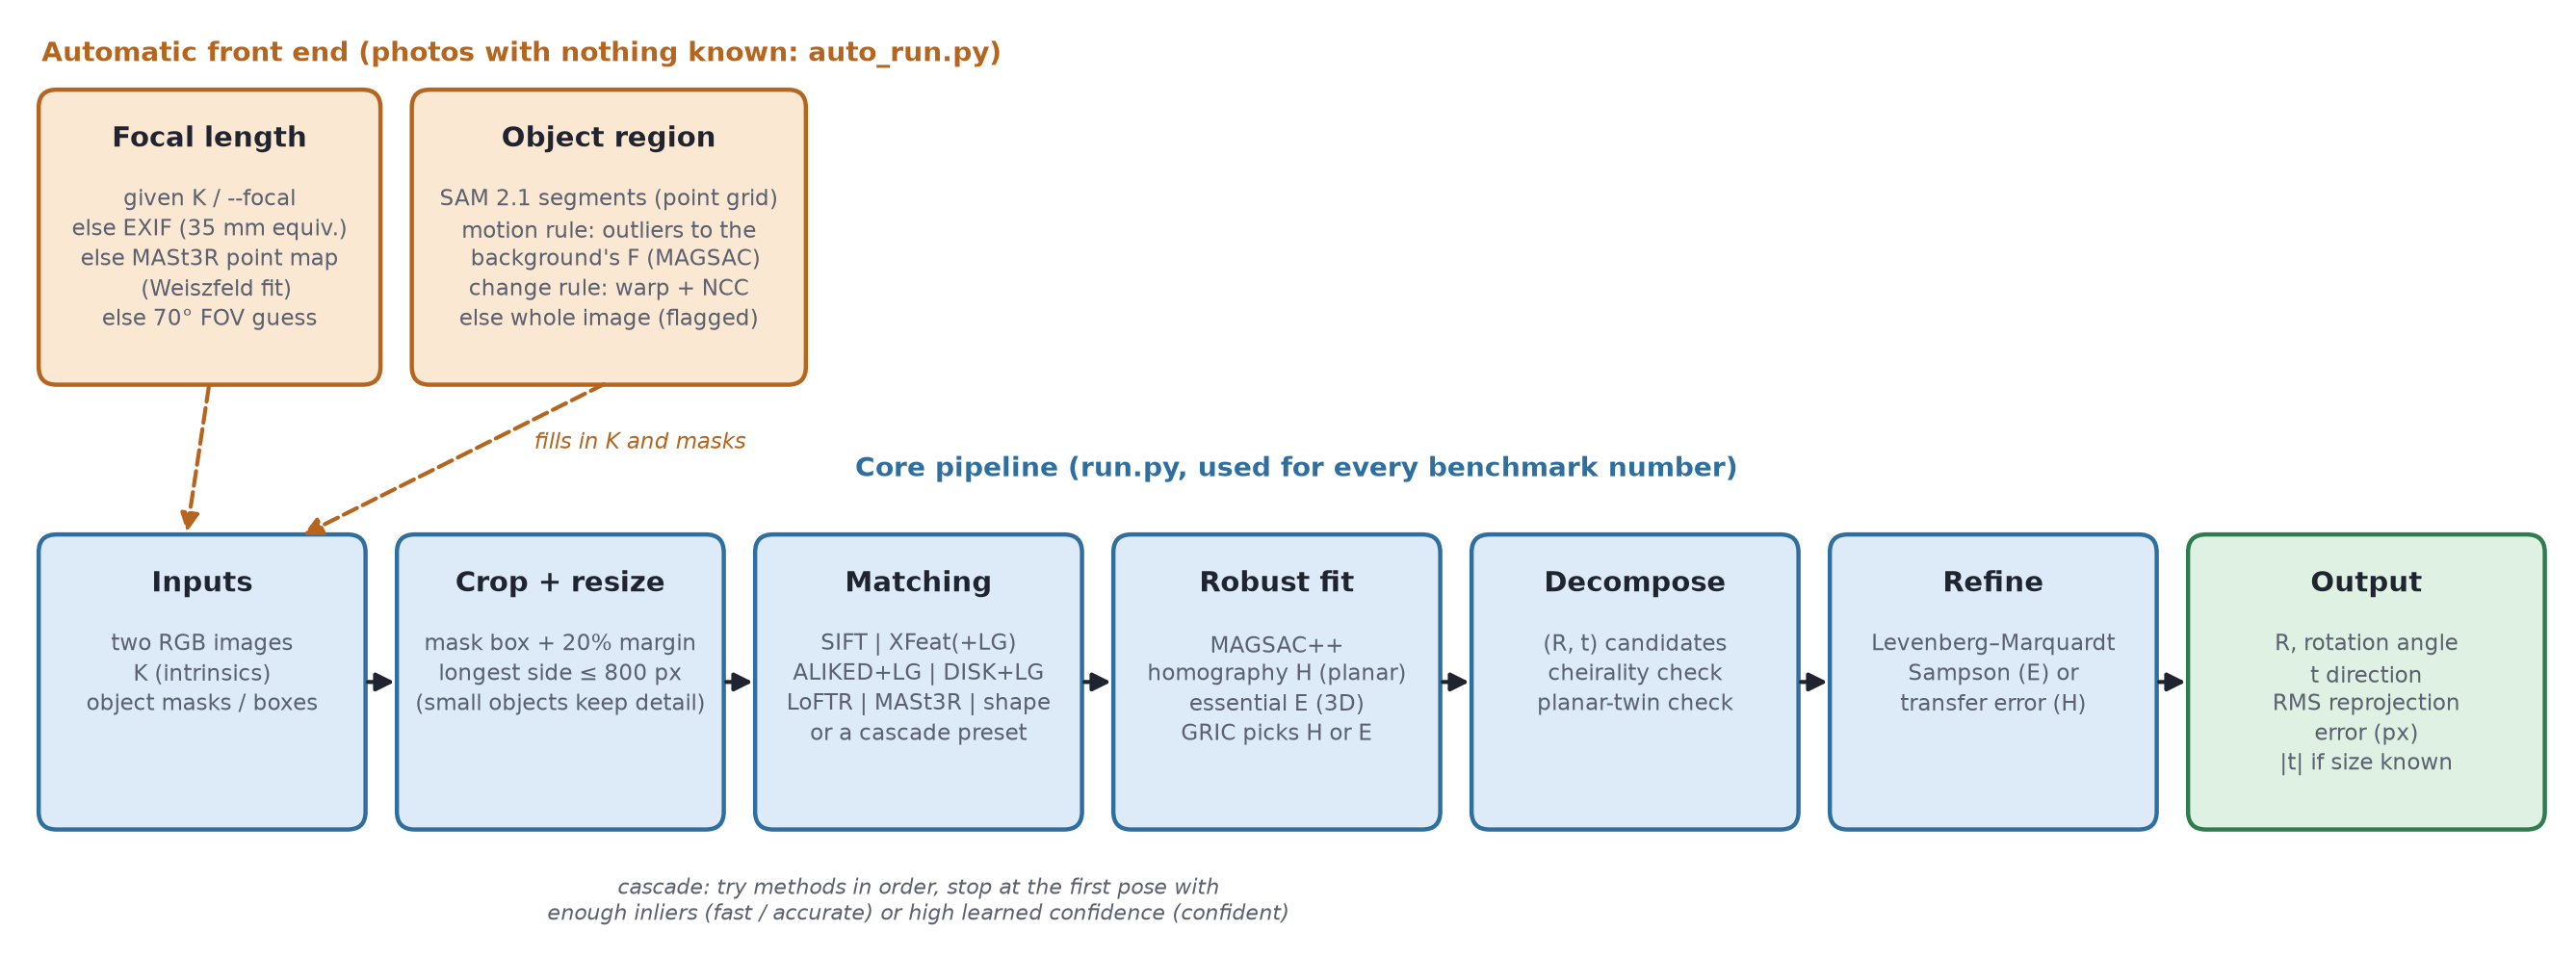
\includegraphics[width=\linewidth]{pipeline.png}
  \caption{The pipeline. Core pipeline: crop around the object, match keypoints, fit a
  homography $H$ and an essential matrix $E$ with MAGSAC++, choose one with GRIC, decompose it
  into $(\R,\tv)$, refine, and report the reprojection error. The automatic front end fills in
  $\K$ and the object masks when they are not given.}
  \label{fig:pipeline}
\end{figure}

The stages are:
\begin{enumerate}
  \item \textbf{Crop and resize.} The bounding box of the object mask is enlarged by 20\% on
        each side and cropped, so a small object fills the image the matcher sees. The crop is
        then shrunk so that its longest side is at most 800\,px (CPU budget). $\K$ is adjusted
        for the crop offset and the scale.
  \item \textbf{Matching.} One matcher (Section~\ref{sec:models}) or a cascade of matchers
        (Section~\ref{sec:presets}) finds correspondences. Only points inside the object mask are kept.
  \item \textbf{Robust model fitting.} Both a homography $H$ and an essential matrix $E$ are
        fitted with MAGSAC++.
  \item \textbf{Model selection.} GRIC picks $H$ or $E$ for each pair.
  \item \textbf{Decomposition.} The chosen model is decomposed into candidate poses. The
        cheirality check keeps the physical one, and the planar-twin check resolves the plane
        ambiguity of $E$.
  \item \textbf{Refinement.} Levenberg--Marquardt minimises a geometric pixel error over all
        inliers.
  \item \textbf{Output.} $\R$, the rotation angle, the direction of $\tv$, the RMS reprojection
        error, and $|\tv|$ in metres if the object's size is given.
\end{enumerate}

% ================================================================ 3
\section{Datasets and preprocessing}
\label{sec:data}

We use four public datasets of real images with ground-truth camera poses
(Table~\ref{tab:datasets}). CO3D and MVImgNet are hundreds of gigabytes each, so only the
needed categories and sequences were downloaded.

\begin{table}[H]
\centering
\small
\setlength{\tabcolsep}{4pt}\begin{tabularx}{\linewidth}{>{\raggedright}p{2.3cm} >{\raggedright}p{3.0cm} X >{\raggedright}p{2.1cm} r}
\toprule
dataset & objects used & ground truth & raw format & test pairs \\
\midrule
TUM RGB-D fr3 \cite{tum} & textured posters (flat / structured, near / far), checkerboard & motion capture, metric & 640$\times$480 image sequence & 142 \\
Objectron \cite{objectron} & book, cereal box, laptop & ARKit poses + 3D boxes, metric & video (.MOV) & 189 \\
CO3Dv2 \cite{co3d} & cellphone, handbag & SfM (COLMAP) poses + masks, scale unknown & image sequence & 210 \\
MVImgNet \cite{mvimgnet} & key, watch & COLMAP poses + cut-out masks, scale unknown & image sequence & 210 \\
\bottomrule
\end{tabularx}
\caption{Datasets. 751 test pairs in total; another 339 pairs were used only for tuning.}
\label{tab:datasets}
\end{table}

\subsection{Per-dataset preprocessing}

All four datasets are converted into the same form: frames with a world-to-camera pose
$(\R_i,\tv_i)$ in the OpenCV convention, a pixel intrinsics matrix $\K_i$ and, where
available, an object mask.

\paragraph{TUM RGB-D.} Five fr3 sequences were downloaded as archives. Only the RGB images
are used (no depth). The motion-capture system gives camera-to-world poses at about 100\,Hz,
while RGB frames arrive at about 30\,Hz, so each frame's pose is \emph{interpolated at its
timestamp}: linearly for the position and by spherical linear interpolation (slerp) for the
rotation quaternion. The poses are then inverted to world-to-camera. The camera axes already
follow OpenCV. In these scenes the textured poster \emph{is} the scene, so the whole image is
used as the object region.

\paragraph{Objectron.} Each sequence is a phone video (\texttt{video.MOV}) plus an
\texttt{annotation.pbdata} file that stores, for every video frame, the ARKit camera pose,
the pixel intrinsics and the 3D bounding box of the object. To get frames:
\begin{enumerate}
  \item The annotation is parsed first, and the pairs to evaluate are chosen from the poses
        (Section~\ref{sec:pairs}).
  \item The video is decoded once with OpenCV, and \emph{only the frames that belong to a chosen
        pair} are written to disk as JPEG (quality 95). Decoding every frame would waste time and space.
  \item The \texttt{.MOV} stores portrait frames (1440$\times$1920), but the intrinsics refer to
        the landscape image (1920$\times$1440), so each frame is rotated by 90$^\circ$ back to landscape.
  \item ARKit cameras use $x$ right, $y$ up, $z$ backward, so poses are converted with
        $F=\mathrm{diag}(1,-1,-1)$. ARKit works in metres, so translations are metric.
  \item The object mask is the filled convex hull of the projected 8 corners of the annotated 3D box.
\end{enumerate}
We used 10 videos per category from Objectron's test split.

\paragraph{CO3Dv2.} A full category is 90--140\,GB. Our downloader reads the remote zip's
central directory and fetches only the needed files with HTTP range requests. Per category it keeps the 10
sequences with the best viewpoint-quality score (at least 100 frames each), and from each
sequence only the RGB images, the object masks and the per-frame cameras. CO3D stores
PyTorch3D cameras (row-vector convention, $x$ left, $y$ up, intrinsics in normalised device
coordinates), converted as
\begin{gather}
  \R_{cv} = F\,\R^\top,\qquad \tv_{cv} = F\,\tv,\qquad F=\mathrm{diag}(-1,-1,1),\\
  f_{px} = f_{ndc}\,s,\qquad c_{px} = (W/2,\,H/2) - p_{ndc}\,s,\qquad s=\min(W,H)/2 .
\end{gather}

\paragraph{MVImgNet.} Each sequence holds about 30 phone frames, a background-removed cut-out
per frame (its alpha channel is the object mask) and a COLMAP sparse model with a
\texttt{SIMPLE\_RADIAL} camera ($f, c_x, c_y, k_1$). Like CO3D, only 10 sequences per category
were fetched by range requests, chosen among those in which COLMAP registered every frame. Images
and masks are undistorted on loading, so the rest of the pipeline sees an ideal pinhole camera.

\subsection{Pair sampling and ground truth}
\label{sec:pairs}

For two frames with world-to-camera poses $(\R_1,\tv_1)$ and $(\R_2,\tv_2)$, the ground-truth
relative pose is
\begin{equation}
  \R_{gt} = \R_2\R_1^\top, \qquad \tv_{gt} = \tv_2 - \R_{gt}\,\tv_1 .
\end{equation}
Pairs are sampled with a fixed random seed and \emph{stratified by viewpoint change}: an equal
number of pairs from each bin of relative rotation, 5--15$^\circ$, 15--30$^\circ$ and
30--60$^\circ$. On TUM the two frames must be at most 3\,s apart, so that they look at the same part
of the scene. Every method is scored on exactly the same pairs.

\paragraph{Checking the conversions.} A wrong axis flip or transpose would silently corrupt every result, so each loader was checked: SIFT matches on sample pairs lie a median of 0.2--3.6\,px from the epipolar lines predicted by the converted ground truth on 25 of 28 sample pairs, against 10--970\,px when $\R$ is deliberately transposed (Appendix, Figure~\ref{fig:check}). The other three are Objectron pairs with 40--53$^\circ$ of viewpoint change, where SIFT itself returns many wrong matches.

\paragraph{Tuning vs.\ test split.} Sequences 01--03 of every object (and the first 30\% of each
TUM video) form the \emph{tuning} split. All thresholds, cascade designs, the confidence model and the
choice of presets were fitted on it. All numbers in this report are on the remaining
\emph{test} pairs.

\paragraph{Image preprocessing at run time.} Each image is cropped to the object's mask box plus a 20\%
margin and resized so that its longest side is at most 800\,px. Both steps are folded into $\K$. No contrast
enhancement is applied: the learned matchers are trained on natural images, and SIFT is
already invariant to affine intensity changes.

% ================================================================ 4
\section{Methods and models}
\label{sec:models}

\subsection{Two-view geometry}
With pixel coordinates normalised by $\K$ ($\hat{\mathbf{x}} = \K^{-1}\mathbf{x}$), a
correspondence of a general 3D point satisfies the epipolar constraint
\begin{equation}
  \hat{\mathbf{x}}_2^\top E\, \hat{\mathbf{x}}_1 = 0, \qquad E = [\tv]_\times \R ,
\end{equation}
and a point on a plane $\mathbf{n}^\top\X_1 = d$ satisfies
\begin{equation}
  \hat{\mathbf{x}}_2 \sim H \hat{\mathbf{x}}_1, \qquad H = \R + \frac{\tv\,\mathbf{n}^\top}{d}.
\end{equation}
$E$ is estimated with the five-point algorithm \cite{nister} and decomposed into four
$(\R,\tv)$ candidates. $H$ is decomposed with Malis and Vargas' method \cite{malis} into up to four
$(\R,\tv,\mathbf{n})$ candidates. The cheirality check keeps the candidate that puts the
triangulated points in front of both cameras.

\subsection{Matchers}

\paragraph{SIFT \cite{sift} (classical).} Keypoints are extrema of a difference-of-Gaussians
scale space. Each is described by a 128-D histogram of gradient orientations, relative to its
dominant orientation, so it is invariant to scale and in-plane rotation. Matches are mutual
nearest neighbours that pass Lowe's ratio test. Fast and rotation-invariant, but it needs texture.

\paragraph{XFeat \cite{xfeat} (learned, sparse).} A very light CNN that detects keypoints and
computes 64-D descriptors, designed for CPUs. It is matched by mutual nearest neighbour.

\paragraph{LightGlue \cite{lightglue} (learned matcher).} A transformer that takes the
keypoints and descriptors of both images and alternates self-attention (within an image) and
cross-attention (across images), then predicts a soft assignment. It stops early on easy pairs.
We pair it with three detectors: \textbf{XFeat+LG}, \textbf{ALIKED+LG} (ALIKED \cite{aliked}
uses deformable convolutions for sub-pixel keypoints) and \textbf{DISK+LG} (DISK \cite{disk} is
trained with reinforcement learning to maximise correct matches).

\paragraph{LoFTR \cite{loftr} (learned, dense, detector-free).} LoFTR does not detect keypoints.
It extracts coarse feature maps from both images, transforms them with interleaved self- and cross-attention,
matches every coarse cell with a dual-softmax, and refines each match at a finer level. Because it
matches everywhere, it finds correspondences on weakly textured surfaces.

\paragraph{MASt3R \cite{mast3r} (3D foundation model).} Built on DUSt3R \cite{dust3r}, a ViT-Large
encoder--decoder that takes both images together and regresses a \emph{3D point map} for each:
the 3D coordinates of every pixel in the first camera's frame. MASt3R adds a dense descriptor
head and is trained to make descriptors of the same 3D point match. Correspondences come from
reciprocal matching of these descriptors. Because the network reasons in 3D, it handles large
viewpoint changes. It is the slowest method here (about 20\,s per pair on CPU).

\paragraph{Shape (outline-only).} For textureless rectangles, such as the back of a phone, there may be
no texture at all. This method fits a quadrilateral to each object mask's outline and estimates
a homography from its four corners. It needs masks and a clean, roughly rectangular outline.

\subsection{Robust estimation and model choice}

\paragraph{MAGSAC++ \cite{magsac}.} RANSAC needs a fixed inlier threshold. MAGSAC++
marginalises over a range of noise scales and weights each point by its likelihood of being an
inlier, which makes it much less sensitive to the threshold. It is used for both $H$ and $E$.

\paragraph{GRIC \cite{gric}.} Neither model is always right: $H$ is better conditioned on flat
objects and small baselines, $E$ is correct for 3D objects. Torr's Geometric Robust Information
Criterion scores both on the same matches,
\begin{equation}
  \mathrm{GRIC} = \sum_i \rho\!\left(\tfrac{e_i^2}{\sigma^2}\right) + \lambda_1\, d\, n + \lambda_2\, k,
  \qquad \rho(x) = \min(x,\; 2(r-d)),
\end{equation}
where $e_i$ is the residual, $d$ the dimension of the model's manifold (2 for $H$, 3 for $E$), $k$
the number of parameters (8 for $H$, 5 for $E$), $r=4$ and $n$ the number of matches. The
lower score wins. Fit is rewarded and complexity penalised.

\paragraph{Planar-twin check.} On a (nearly) flat object, a plane's homography has two physically
valid decompositions. Both explain every point on the plane, and $E$-estimation can return
either one; we observed this live, with 2--5$^\circ$ returned for a true rotation of 28--68$^\circ$. When GRIC
picks $E$, we compute the plane's homography from the inliers and its decompositions. If $E$'s
pose coincides with a candidate that is physically impossible, or with the less likely of the
two valid twins (by Sampson error, then by the prior that the plane faces both cameras), it is replaced.
The replacement is accepted only if it fits all matches within $3\times$ $E$'s own Sampson error,
which protects real 3D objects. The factor 3 was set on the tuning split.

\paragraph{Refinement.} Levenberg--Marquardt minimises a geometric pixel error over all inliers,
and the result is kept only if it lowers the median error. For $E$, the cost is the Sampson
distance over 5 parameters (axis-angle rotation and $\tv$ on the unit sphere). For $H$, it is the
symmetric transfer error over $\R$, $\tv/d$ and $\mathbf{n}$, so the result stays a rigid motion.

\paragraph{Reprojection error.} The inliers are triangulated with the final $(\R,\tv)$ and reprojected
into both images. We report the RMS pixel error over the points in front of both cameras.

\subsection{Confidence model}
A gradient-boosted tree classifier \cite{sklearn} predicts, for a pose from a given matcher, the
probability that its error is below $10^\circ$. Its inputs are the number of matches and inliers,
the inlier ratio, the reprojection error, the GRIC margin between $H$ and $E$, and the agreement
between the poses of the matchers already run. It was trained on the tuning split only, with
out-of-fold predictions so that its training pairs never score themselves.

\subsection{Presets: \texttt{fast}, \texttt{accurate}, \texttt{confident}}
\label{sec:presets}

No single matcher is best on every object, so the pipeline offers \emph{cascades}. A cascade runs
methods in order and stops at the first one whose pose it trusts (Figure~\ref{fig:cascades}).
The order and the thresholds were chosen by an exhaustive search (268\,k designs for the inlier
cascades, 4\,368 for the confidence cascades) on the tuning split only.

\begin{itemize}
  \item \textbf{\texttt{fast}}: XFeat+LG, accepted at $\ge 30$ inliers; else SIFT, accepted at
        $\ge 15$; else the outline method. About 0.8\,s per pair.
  \item \textbf{\texttt{accurate}}: XFeat+LG, accepted at $\ge 200$ inliers; else the outline
        method; else SIFT at $\ge 50$; else LoFTR at $\ge 120$. Median 1.1\,s, mean 3.0\,s,
        because LoFTR runs only on the pairs where the cheaper stages fail.
  \item \textbf{\texttt{confident}}: XFeat+LG, then SIFT, then the outline method, each accepted only if
        the \emph{learned confidence} is at least 0.45. Otherwise MASt3R gives the answer. Most
        pairs stop after XFeat+LG; about a quarter go on to MASt3R. Median 0.7\,s, mean 7.8\,s.
\end{itemize}

\begin{figure}[H]
  \centering
  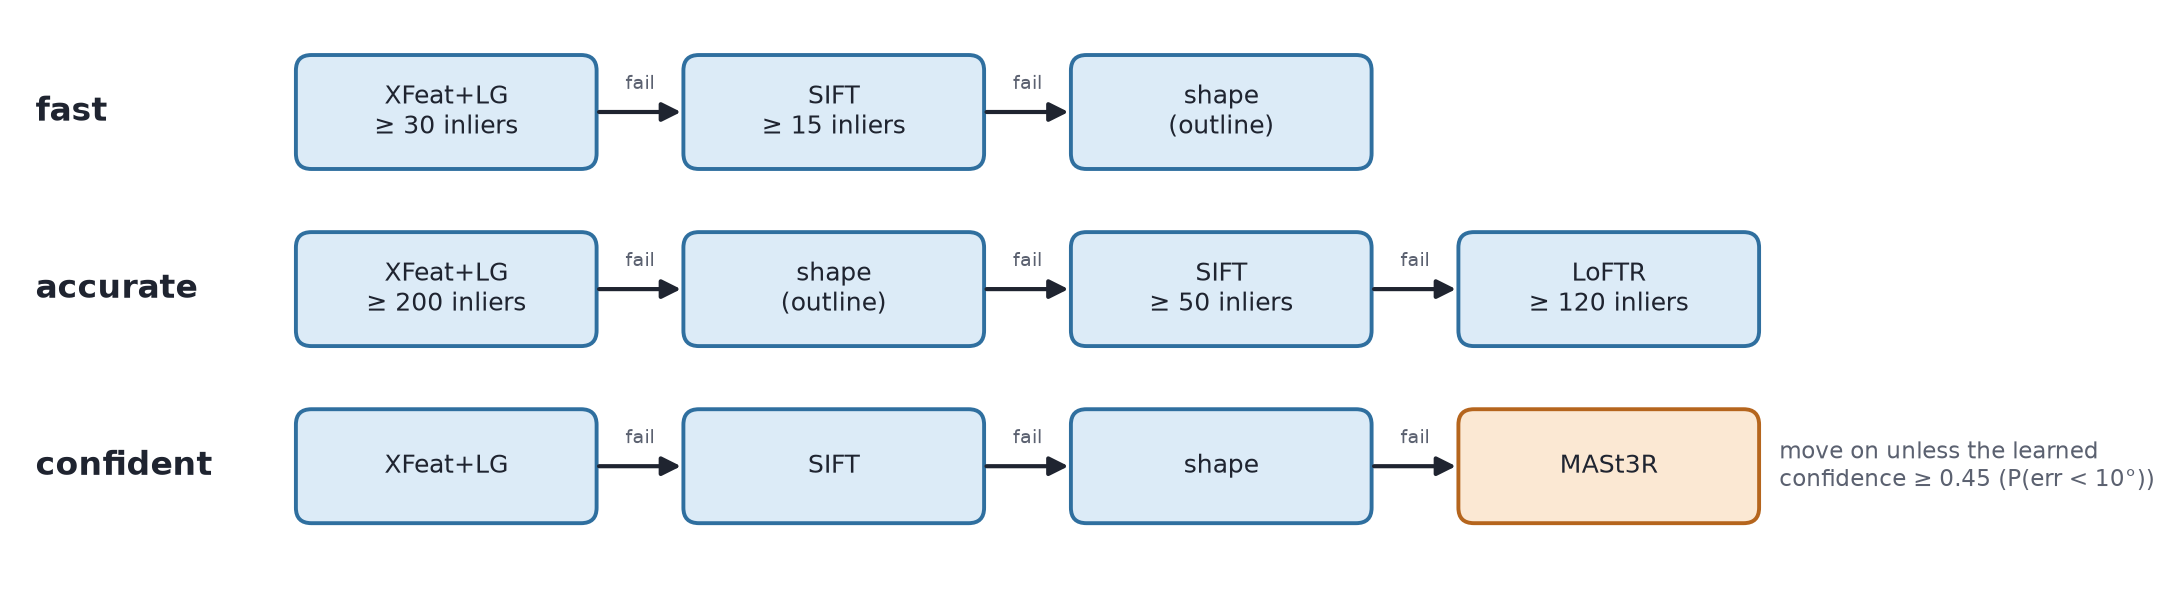
\includegraphics[width=0.95\linewidth]{cascades.png}
  \caption{The three cascade presets. Each box is tried only if the one before it is not trusted.
  \texttt{fast} and \texttt{accurate} trust a stage by its inlier count; \texttt{confident} trusts it by the
  learned probability that its error is below $10^\circ$.}
  \label{fig:cascades}
\end{figure}

\subsection{Automatic front end (unknown photographs)}
\label{sec:auto}

\paragraph{Focal length.} Tried in this order: (1) a given $\K$ or focal length; (2) the
EXIF 35\,mm-equivalent focal length $f_{35}$, converted as
$f_{px} = f_{35}\,\sqrt{W^2+H^2}\,/\,43.27$ (43.27\,mm is the diagonal of a 35\,mm frame); (3)
an estimate from MASt3R's point map; (4) a 70$^\circ$ field-of-view guess, flagged in the
output. For (3), MASt3R predicts a 3D point $(X,Y,Z)$ for every pixel $(u,v)$ in the camera's own
frame. With the principal point $(c_x,c_y)$ at the image centre, the focal length is the
value that best projects the points back to their pixels,
\begin{equation}
  f^\ast = \arg\min_f \sum_{u,v} \left\| (u-c_x,\;v-c_y) - f\,(X/Z,\;Y/Z) \right\|,
\end{equation}
solved robustly by Weiszfeld iterations. The estimates from both images are averaged when the images are the same size.
The principal point is put at the image centre.

\paragraph{Object region.} SAM~2.1 \cite{sam2} (tiny), prompted with a grid of points, splits each
image into candidate segments; segments that touch the border or are tiny are dropped. Two rules
decide which segment is the object:
\begin{itemize}
  \item \textbf{Motion rule.} XFeat+LG matches the whole images. The matches outside all candidates
        (the background) give a fundamental matrix $F_{bg}$ (MAGSAC). A candidate whose matches are
        mostly \emph{outliers} to $F_{bg}$, i.e.\ an outlier share at least 50 percentage points above the background's own,
        moved differently from the background and is the object.
  \item \textbf{Change rule.} When a moved object has too few matches (a rotated key), the
        background around the segment is warped from image 1 to image 2 by a local homography, and the
        normalised cross-correlation is compared inside the segment and in a ring around it. A
        segment whose content changed while its surrounding ring stayed similar is the object.
\end{itemize}
The same object in image 2 is found by voting with the matches. If no object is confirmed, the
whole image is used and the output says so.

\paragraph{Verdict.} Each result is labelled \textsc{reliable}, \textsc{uncertain} (fewer than 30
inliers, reprojection error above 2\,px, or a guessed focal length) or \textsc{no result}.

% ================================================================ 5
\section{Evaluation protocol}

\begin{itemize}
  \item \textbf{Rotation error:} the angle of the residual rotation,
        \[e_R = \arccos\!\big((\mathrm{tr}(\R_{est}^\top\R_{gt})-1)/2\big).\]
  \item \textbf{Translation-direction error:} the angle between the directions,
        \[e_t = \arccos\!\big(\tv_{est}^\top\tv_{gt} / (\|\tv_{est}\|\,\|\tv_{gt}\|)\big).\] Scale is ignored.
  \item \textbf{Pose error} $= \max(e_R, e_t)$.
  \item \textbf{AUC@5/10/20}: the area under the curve of ``share of pairs with pose error below
        $x$'' for $x$ from 0 up to 5, 10 and 20$^\circ$, normalised to 100\%. This is the standard
        relative-pose measure of SuperGlue \cite{superglue} and LoFTR \cite{loftr}. \emph{Failed pairs
        count as infinite error}, so a method cannot gain by refusing hard pairs.
  \item \textbf{Failure rate}, median rotation and translation-direction errors over solved pairs,
        median RMS reprojection error, and seconds per pair on the laptop CPU.
  \item \textbf{Object only:} matches come only from the object's mask, which is the task.
        Using the whole image is reported separately as ``with surroundings''.
\end{itemize}

% ================================================================ 6
\section{Results}

\subsection{Main result}

Table~\ref{tab:main} gives the main result on all 751 test pairs. The full table with every
matcher and AUC@5/20 is in Appendix~\ref{app:full}.

\begin{table}[H]
\centering
\small
\setlength{\tabcolsep}{4pt}\begin{tabular}{l rrrr r r rr r}
\toprule
 & \multicolumn{5}{c}{AUC@10 (\%)} & & \multicolumn{2}{c}{median error ($^\circ$)} & \\
\cmidrule(lr){2-6}\cmidrule(lr){8-9}
method & TUM & Objectron & CO3D & MVImgNet & \textbf{mean} & failed & rot & t-dir & s/pair \\
\midrule
SIFT & 65.8 & 50.7 & 18.1 & 8.5 & 35.8 & 40\% & 1.22 & 2.62 & 0.1 \\
XFeat+LightGlue & 67.2 & 58.2 & 32.0 & 28.3 & 46.4 & 8\% & 1.82 & 3.40 & 0.5 \\
LoFTR & 67.1 & 65.2 & 33.1 & 24.4 & 47.5 & 9\% & 1.41 & 3.12 & 5.4 \\
MASt3R & \best{76.8} & \best{81.5} & \best{67.8} & \best{65.9} & \best{73.0} & 0\% & \best{0.90} & \best{1.49} & 20.2 \\
\midrule
cascade \texttt{fast} & 67.8 & 60.9 & 35.5 & 28.3 & 48.1 & 4\% & 1.86 & 3.61 & 0.7 \\
cascade \texttt{accurate} & 68.1 & 63.0 & 38.6 & 30.2 & 50.0 & 3\% & 1.78 & 3.37 & 0.9 \\
cascade \texttt{confident} & 70.5 & 77.2 & 57.4 & 51.1 & 64.0 & 0\% & 1.21 & 1.91 & 0.8 \\
\bottomrule
\end{tabular}
\caption{Relative pose of the object, test split, object only. Failed pairs count as infinite
error. Seconds are medians on a laptop CPU.}
\label{tab:main}
\end{table}

\begin{figure}[H]
  \centering
  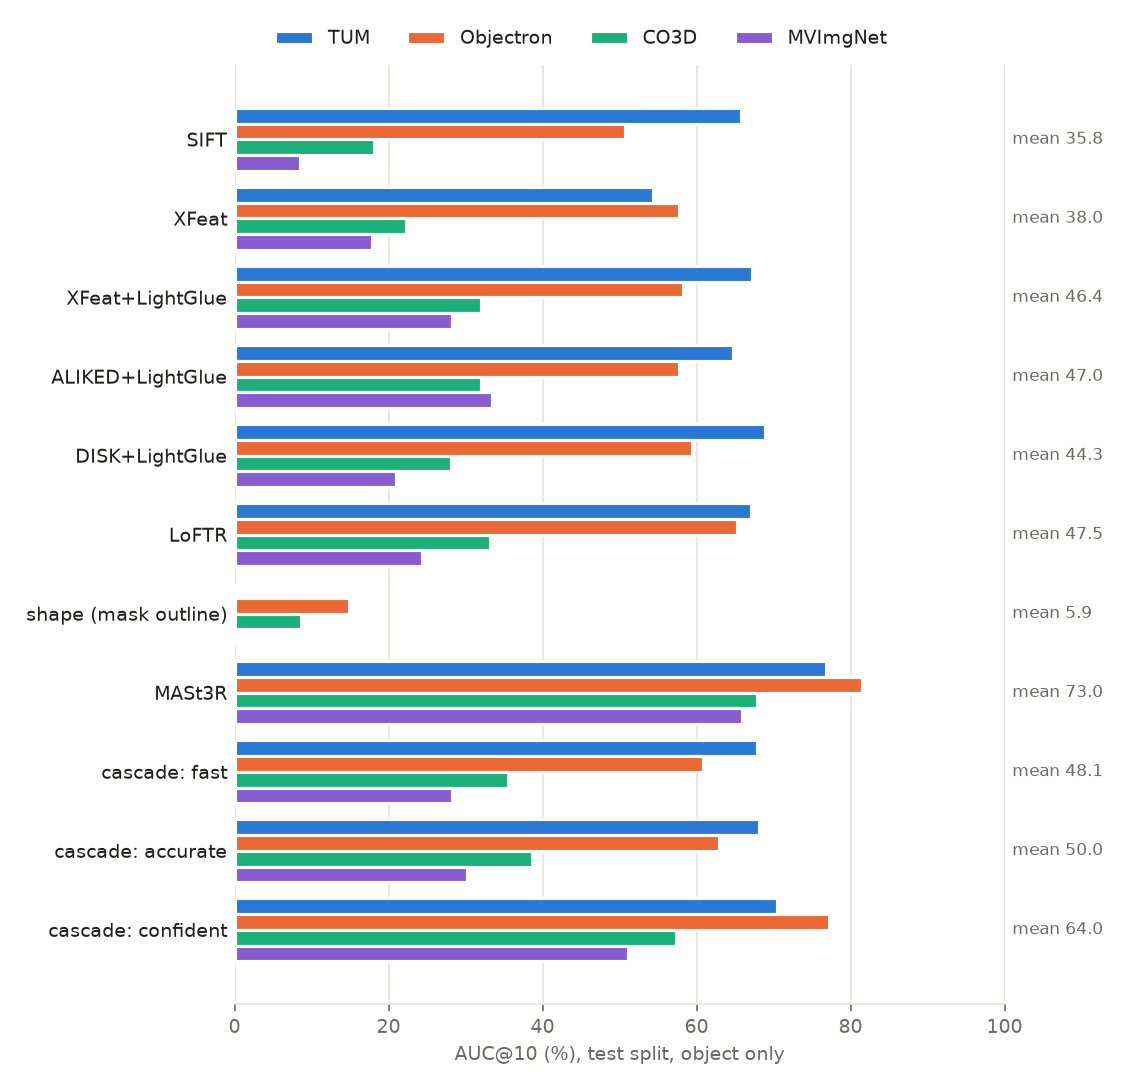
\includegraphics[width=0.6\linewidth]{overview.png}
  \caption{AUC@10 per method and dataset (test split, object only).}
  \label{fig:overview}
\end{figure}

\paragraph{Observations.}
\begin{itemize}
  \item \textbf{MASt3R is the most accurate method} on every dataset, with sub-degree median
        rotation error and no failures. It was trained on CO3D, but its gain over the best
        other method is as large on MVImgNet (+32 points), which it never saw, as on CO3D (+35), so the
        advantage is not memorisation.
  \item \textbf{Learned sparse matchers beat SIFT on the hard sets} (phones in CO3D, keys and
        watches in MVImgNet), where SIFT fails on 40\% of pairs. On well-textured planar scenes
        (TUM) SIFT is still competitive.
  \item \textbf{The cascades beat every single matcher except MASt3R.} \texttt{accurate} (50.0) is
        above LoFTR (47.5) at about a sixth of its time.
  \item \textbf{\texttt{confident} is the best accuracy per second.} It sends only the doubtful
        quarter of pairs to MASt3R and gets most of MASt3R's accuracy at a median of 0.7\,s. It also
        accepts far fewer wrong answers: 7\% of test pairs end more than 20$^\circ$ off, against 19--21\%
        for cascades that use the cheap matchers only.
  \item \textbf{Reprojection error} of the inliers is 0.4--0.6\,px (median) for every matcher, and
        0.29\,px for MASt3R.
  \item \textbf{The hardest objects} are keys and phones: tiny, shiny and with few features.
\end{itemize}

\subsection{Planar or 3D model: homography, essential matrix or GRIC?}
With the same ALIKED+LightGlue matches and only the geometric model changed:

\begin{table}[H]
\centering
\small
\begin{tabular}{l r l}
\toprule
model & AUC@10, all test pairs & remark \\
\midrule
homography $H$ only & 29.9 & best on distant flat posters (55.5) \\
essential matrix $E$ only & 44.3 & only 18.6 on distant flat posters \\
GRIC choice per pair & \best{44.9} & beats both overall; chose $H$ on 17\% of pairs \\
\bottomrule
\end{tabular}
\caption{Model choice (ALIKED+LightGlue, test split).}
\end{table}

Before the planar-twin check, $E$ scored only 5.8 on the distant flat posters, because it returned the
wrong twin. The check raised every matcher's mean AUC@10 by 1--3 points, and XFeat+LightGlue on
Objectron by 9 (49.3 $\to$ 58.2); no dataset lost more than 0.3.

\subsection{Object only vs.\ with surroundings}

\begin{table}[H]
\centering
\small
\begin{tabular}{l l rrrr}
\toprule
method & input & TUM & Objectron & CO3D & MVImgNet \\
\midrule
ALIKED+LG & object only & 64.7 & 57.8 & 32.1 & 33.5 \\
ALIKED+LG & with surroundings & 64.7 & 77.1 & 72.0 & 74.9 \\
SIFT & object only & 65.8 & 50.7 & 18.1 & 8.5 \\
SIFT & with surroundings & 65.8 & 63.4 & 45.8 & 44.8 \\
\bottomrule
\end{tabular}
\caption{AUC@10 (\%) with matches restricted to the object vs.\ the whole image (TUM is the whole image in both).}
\end{table}

Using the whole image looks much better, but it measures the \emph{camera's} motion against the static
background. In these datasets the object never moves relative to the scene, so the two coincide; for an object
that is moved by hand they do not. All main results are therefore object only.

\subsection{Accuracy vs.\ viewpoint change}

\begin{table}[H]
\centering
\small
\begin{tabular}{l rrr}
\toprule
method & 5--15$^\circ$ & 15--30$^\circ$ & 30--60$^\circ$ \\
\midrule
SIFT & 40.2 & 35.7 & 19.2 \\
XFeat+LG & 47.1 & 52.6 & 30.3 \\
ALIKED+LG & 49.6 & 50.9 & 32.2 \\
LoFTR & 53.4 & 52.3 & 26.1 \\
MASt3R & \best{68.3} & \best{76.5} & \best{72.4} \\
\bottomrule
\end{tabular}
\caption{AUC@10 (\%) per bin of true rotation, all datasets.}
\end{table}

Between 30 and 60$^\circ$ every 2D matcher drops to 19--32 points, while MASt3R stays at 72.

\subsection{Sensitivity to errors in $\K$}

Using the same matches with a deliberately wrong $\K$ (XFeat+LightGlue, mean AUC@10):
a focal-length error of $\pm2\%$ costs about 1 point, $\pm5\%$ about 2, and $\pm10\%$ about 6 (46.4 $\to$ 40.6).
The principal point matters more: shifting it by 5\% of the image size costs 7.6 points, and by 10\% the
AUC almost halves (26.9).

\begin{figure}[H]
  \centering
  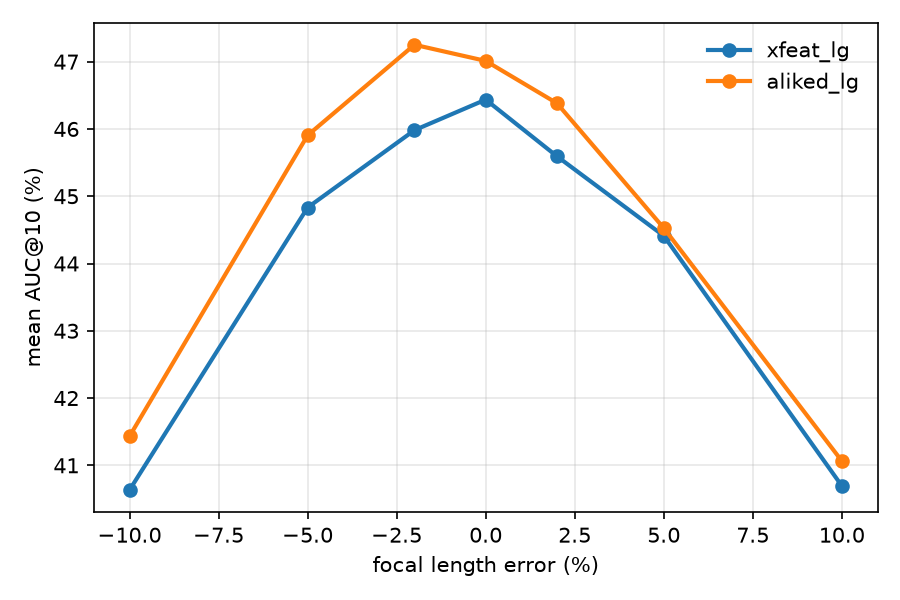
\includegraphics[width=0.6\linewidth]{focal_sens.png}
  \caption{AUC@10 against the error in the focal length.}
\end{figure}

\paragraph{Calibration.} Zhang's method \cite{zhang} on TUM's checkerboard sequence (262 views, no
distortion terms) gives a focal length within 2.3\% of TUM's official value, with a corner RMS error
of 0.22\,px. This is well within the tolerance above. A low corner error alone does not prove a good
$\K$, though: a $\K$ that is 28\% off reprojected held-out views almost as well (0.230 vs.\ 0.219\,px), because
this board is nearly always seen face-on.

\subsection{Metric scale}
\label{sec:scale}
Two views give $\tv$ only up to scale. If the object's longest side is known, the triangulated
inliers' extent along their main axis is matched to that length. On Objectron this recovers
$|\tv|$ with a median error of 17.9\%, with 59\% of pairs within 25\%. MASt3R's metric depth was off by
a median factor of about 1.5 on TUM and 3 on Objectron close-ups, so it is not used for scale.

\subsection{Run time}

\begin{table}[H]
\centering
\small
\begin{tabular}{l rr}
\toprule
method & median s/pair & mean s/pair \\
\midrule
SIFT & 0.13 & 0.28 \\
XFeat+LightGlue & 0.56 & 0.61 \\
ALIKED+LightGlue & 1.8 & 1.7 \\
DISK+LightGlue & 4.7 & 4.4 \\
LoFTR & 5.8 & 6.6 \\
MASt3R & 23.7 & 23.6 \\
\texttt{fast} & 0.80 & 0.83 \\
\texttt{accurate} & 1.1 & 3.0 \\
\texttt{confident} & $\approx$0.7 & $\approx$7.8 \\
\bottomrule
\end{tabular}
\caption{Run time on a laptop CPU (same 24 pairs, one session).}
\end{table}

\subsection{Blind setting: no intrinsics and no object region}

At a demonstration the photographs come with neither $\K$ nor a mask. We measured the cost of the
automatic front end (Section~\ref{sec:auto}) on random test pairs, all with MASt3R for the pose:
\textbf{A} uses the dataset $\K$ and region; \textbf{B} replaces $\K$ by the MASt3R focal estimate
with the principal point at the centre; \textbf{D} also finds the region automatically, with no
object name.

\begin{table}[H]
\centering
\small
\begin{tabular}{l rrr}
\toprule
version & TUM (20 pairs) & Objectron (15) & CO3D (16) \\
\midrule
A: dataset $\K$, dataset region & 76.4 & 84.8 & 67.9 \\
B: estimated focal, dataset region & 71.7 & 80.3 & 61.0 \\
D: estimated focal, automatic region & 71.7 & 80.4 & 74.8 \\
\midrule
focal estimate, median $|$error$|$ & 4.4\% & 3.2\% & 3.0\% \\
\bottomrule
\end{tabular}
\caption{AUC@10 (\%) without known intrinsics or regions (MASt3R pose).}
\label{tab:blind}
\end{table}

The fully automatic version loses 4--5 points on TUM and Objectron. On CO3D it gains, because the
automatic region often includes surroundings that move with the camera. These runs used the region
finder before the change rule was added.

\subsection{Our own photographs}

We photographed small objects with an iPhone 16 Pro Max (24\,mm main lens). The images had no EXIF
data, so the focal length came from the 35\,mm equivalent ($\approx$1110\,px at 1200$\times$1600) or
from the MASt3R estimate, and the region was found automatically. The object was turned by hand
on a surface, by a roughly known angle.

\begin{table}[H]
\centering
\small
\begin{tabularx}{\linewidth}{l c c c X}
\toprule
object & true turn & \texttt{accurate} & \texttt{mast3r} & remark \\
\midrule
coin & $\approx45^\circ$ & \best{47.2$^\circ$} & 18.1$^\circ$ & SIFT answered: 69 of 78 matches agree, 0.16\,px; axis $(0.00,-0.49,-0.87)$, a turn about the surface normal. MASt3R's axis is the camera $x$ axis (a tipping motion). \\
key & $\approx55$--$60^\circ$ & \best{50$^\circ$} & 16.8$^\circ$ & region found by the change rule; SIFT-like matches tooth to tooth. \\
wallet & $\approx45^\circ$ & -- & \best{40.6$^\circ$} & dark, low texture; MASt3R correct. \\
mouse & $\approx60^\circ$ & 7$^\circ$ & 13$^\circ$ & region not found, so the whole image was used; both measure the camera's motion. \\
\bottomrule
\end{tabularx}
\caption{Own photographs (no ground truth beyond the approximate turn).}
\label{tab:own}
\end{table}

\begin{figure}[H]
  \centering
  \begin{subfigure}{0.49\linewidth}
    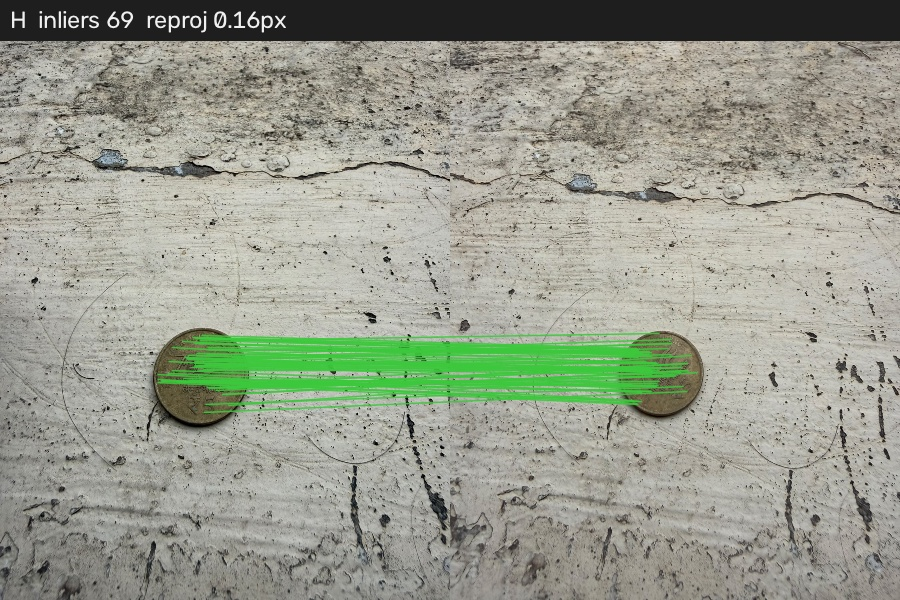
\includegraphics[width=\linewidth]{coin_accurate.jpg}
    \caption{coin, \texttt{accurate}: 47.2$^\circ$}
  \end{subfigure}
  \hfill
  \begin{subfigure}{0.49\linewidth}
    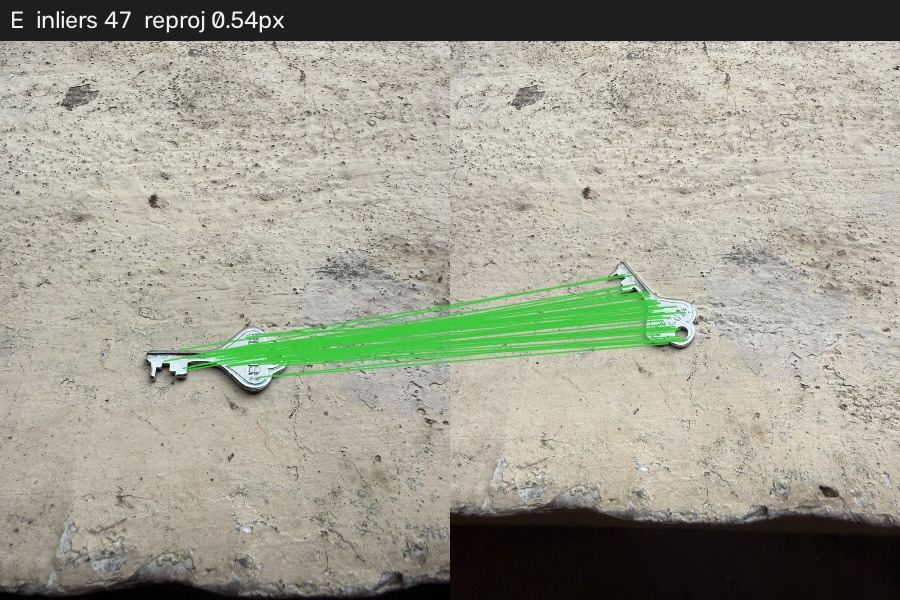
\includegraphics[width=\linewidth]{key_accurate.jpg}
    \caption{key, \texttt{accurate}: 50$^\circ$}
  \end{subfigure}
  \caption{Inlier matches on our own photographs.}
\end{figure}

The pattern is clear: \textbf{MASt3R underestimates large in-plane turns}. Its matches pair points as if
the object had barely turned, while the rotation-invariant SIFT descriptor follows the turn. Both
answers have low reprojection errors, so the reprojection error alone cannot tell them apart.
The direction of the rotation axis can: an object turned flat on a surface must rotate about the
surface's normal.

% ================================================================ 7
\section{Limitations}
\begin{itemize}
  \item Two views give $\tv$ only up to scale; a known object size gives about 18\% error.
  \item Without texture (plain phone backs, dark watch faces) matching fails. The outline method helps
        only for clean rectangles.
  \item MASt3R is accurate on viewpoint changes but slow on CPU, and it misses large in-plane rotations
        of a flat object. Its wrong answers are self-consistent, so they still look reliable.
  \item The pose depends on $\K$. The MASt3R focal estimate is 3--4\% off on the datasets but 15--27\%
        off on close-up phone photos.
  \item The automatic region finder can miss an object that barely changes appearance (the mouse), and
        then falls back to the whole image, which measures the camera's motion.
  \item Objectron's masks are projected 3D boxes, not silhouettes, which hurts the outline method there.
\end{itemize}

% ================================================================ 8
\section{Conclusion}
We built and evaluated a CPU-only pipeline that estimates the change in 3D pose of a small object
from two RGB images, together with its reprojection error. On 751 held-out pairs from four real-image
datasets, the 3D foundation model MASt3R is the most accurate (AUC@10 73.0\%, median rotation error
0.90$^\circ$). A confidence-gated cascade keeps most of that accuracy (64.0\%) at a median of 0.7\,s per pair,
and the inlier cascades \texttt{fast} and \texttt{accurate} beat every single classical or learned 2D matcher.
GRIC with a planar-twin check handles both flat and 3D objects. For unknown photographs, an automatic
front end estimates the focal length and finds the object, at a cost of 4--5 AUC points. Tests on our
own photographs show that the rotation-invariant classical SIFT still wins for large in-plane turns, which
suggests running both kinds of matcher and checking the rotation axis against the supporting surface.

% ---------------------------------------------------------------- references
\begin{thebibliography}{99}\small
\bibitem{tum} J. Sturm, N. Engelhard, F. Endres, W. Burgard, D. Cremers. A benchmark for the evaluation of RGB-D SLAM systems. IROS, 2012.
\bibitem{objectron} A. Ahmadyan, L. Zhang, A. Ablavatski, J. Wei, M. Grundmann. Objectron: A large scale dataset of object-centric videos in the wild with pose annotations. CVPR, 2021.
\bibitem{co3d} J. Reizenstein, R. Shapovalov, P. Henzler, L. Sbordone, P. Labatut, D. Novotny. Common Objects in 3D. ICCV, 2021.
\bibitem{mvimgnet} X. Yu et al. MVImgNet: A large-scale dataset of multi-view images. CVPR, 2023.
\bibitem{sift} D. G. Lowe. Distinctive image features from scale-invariant keypoints. IJCV, 60(2), 2004.
\bibitem{xfeat} G. Potje, F. Cadar, A. Araujo, R. Martins, E. R. Nascimento. XFeat: Accelerated features for lightweight image matching. CVPR, 2024.
\bibitem{lightglue} P. Lindenberger, P.-E. Sarlin, M. Pollefeys. LightGlue: Local feature matching at light speed. ICCV, 2023.
\bibitem{aliked} X. Zhao et al. ALIKED: A lighter keypoint and descriptor extraction network via deformable transformation. IEEE TIM, 2023.
\bibitem{disk} M. Tyszkiewicz, P. Fua, E. Trulls. DISK: Learning local features with policy gradient. NeurIPS, 2020.
\bibitem{loftr} J. Sun, Z. Shen, Y. Wang, H. Bao, X. Zhou. LoFTR: Detector-free local feature matching with transformers. CVPR, 2021.
\bibitem{dust3r} S. Wang, V. Leroy, Y. Cabon, B. Chidlovskii, J. Revaud. DUSt3R: Geometric 3D vision made easy. CVPR, 2024.
\bibitem{mast3r} V. Leroy, Y. Cabon, J. Revaud. Grounding image matching in 3D with MASt3R. ECCV, 2024.
\bibitem{superglue} P.-E. Sarlin, D. DeTone, T. Malisiewicz, A. Rabinovich. SuperGlue: Learning feature matching with graph neural networks. CVPR, 2020.
\bibitem{magsac} D. Barath, J. Noskova, M. Ivashechkin, J. Matas. MAGSAC++, a fast, reliable and accurate robust estimator. CVPR, 2020.
\bibitem{gric} P. H. S. Torr. Geometric motion segmentation and model selection. Phil. Trans. Royal Society A, 1998.
\bibitem{nister} D. Nist\'er. An efficient solution to the five-point relative pose problem. IEEE TPAMI, 26(6), 2004.
\bibitem{malis} E. Malis, M. Vargas. Deeper understanding of the homography decomposition for vision-based control. INRIA RR-6303, 2007.
\bibitem{hz} R. Hartley, A. Zisserman. Multiple View Geometry in Computer Vision. Cambridge University Press, 2nd ed., 2004.
\bibitem{zhang} Z. Zhang. A flexible new technique for camera calibration. IEEE TPAMI, 22(11), 2000.
\bibitem{sam2} N. Ravi et al. SAM 2: Segment anything in images and videos. arXiv:2408.00714, 2024.
\bibitem{sklearn} F. Pedregosa et al. Scikit-learn: Machine learning in Python. JMLR, 12, 2011.
\end{thebibliography}

% ---------------------------------------------------------------- appendix
\appendix
\section{Full results}
\label{app:full}

\begin{table}[H]
\centering
\small
\scriptsize\setlength{\tabcolsep}{3pt}\begin{tabular}{l l rrrr r}
\toprule
method & kind & TUM & Objectron & CO3D & MVImgNet & failed \\
\midrule
SIFT & classical & 50.3 / 65.8 / 77.0 & 37.9 / 50.7 / 60.5 & 12.1 / 18.1 / 22.7 & 4.2 / 8.5 / 13.2 & 40\% \\
XFeat & learned sparse & 36.6 / 54.3 / 69.9 & 43.3 / 57.7 / 67.9 & 13.5 / 22.3 / 33.4 & 9.5 / 17.8 / 28.5 & 5\% \\
XFeat+LG & learned sparse & 49.7 / 67.2 / 79.2 & 44.9 / 58.2 / 67.9 & 21.5 / 32.0 / 42.7 & 16.1 / 28.3 / 40.3 & 8\% \\
ALIKED+LG & learned sparse & 47.6 / 64.7 / 76.5 & 44.2 / 57.8 / 67.1 & 22.6 / 32.1 / 39.9 & 19.0 / 33.5 / 46.6 & 18\% \\
DISK+LG & learned sparse & 52.5 / 68.9 / 80.0 & 46.8 / 59.5 / 66.9 & 21.2 / 28.1 / 34.2 & 10.9 / 21.0 / 31.2 & 21\% \\
LoFTR & learned dense & 51.7 / 67.1 / 76.8 & 50.9 / 65.2 / 74.6 & 24.1 / 33.1 / 43.1 & 13.9 / 24.4 / 35.1 & 9\% \\
shape & outline & 0.0 / 0.0 / 0.0 & 10.4 / 14.9 / 22.8 & 2.9 / 8.6 / 16.0 & 0.0 / 0.0 / 0.0 & 72\% \\
MASt3R & 3D model & 60.2 / 76.8 / 86.9 & 66.3 / 81.5 / 90.2 & 47.4 / 67.8 / 82.2 & 44.1 / 65.9 / 79.8 & 0\% \\
\texttt{fast} & cascade & 50.3 / 67.8 / 79.9 & 47.2 / 60.9 / 71.1 & 22.5 / 35.5 / 47.9 & 16.1 / 28.3 / 40.3 & 4\% \\
\texttt{accurate} & cascade & 50.3 / 68.1 / 80.7 & 49.0 / 63.0 / 72.8 & 24.2 / 38.6 / 53.1 & 17.2 / 30.2 / 43.1 & 3\% \\
\texttt{confident} & cascade & 52.3 / 70.5 / 83.3 & 61.6 / 77.2 / 87.5 & 38.1 / 57.4 / 72.2 & 31.7 / 51.1 / 66.5 & 0\% \\
\bottomrule
\end{tabular}
\caption{AUC@5 / @10 / @20 (\%) per dataset, test split, object only.}
\end{table}

\begin{figure}[H]
  \centering
  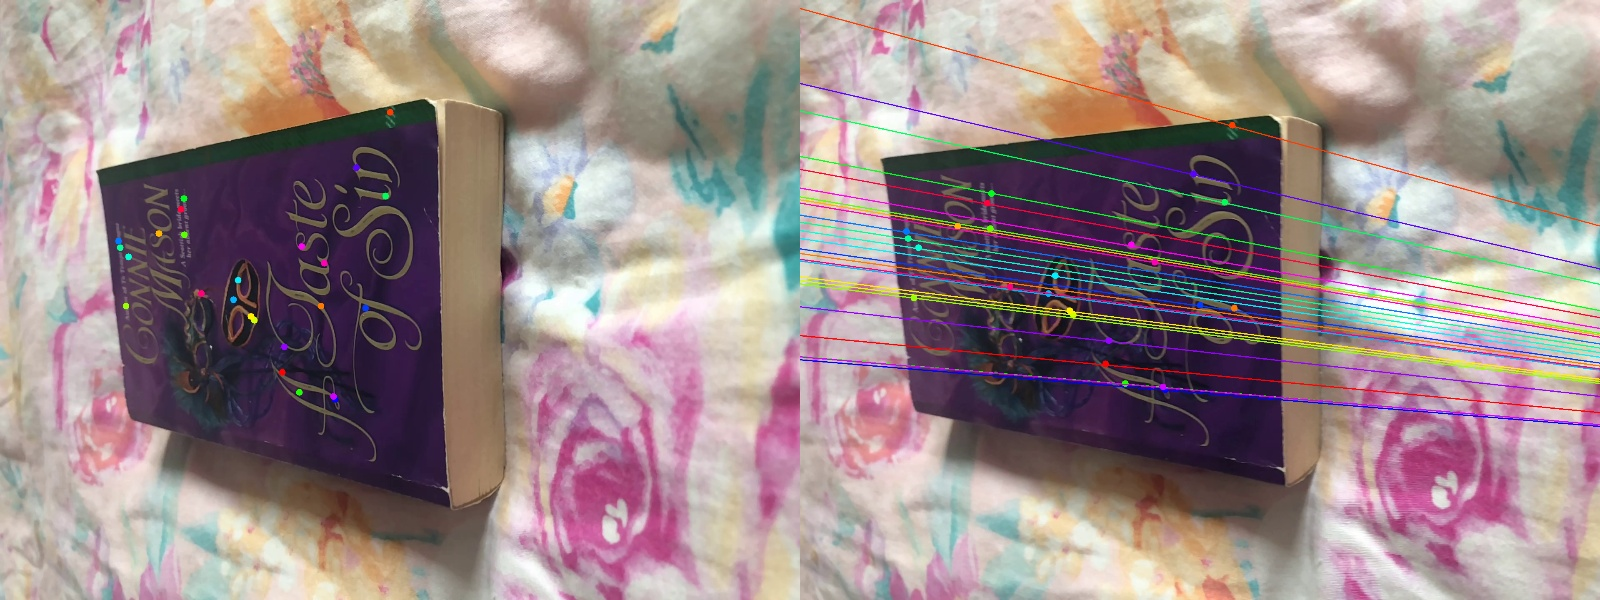
\includegraphics[width=0.85\linewidth]{objectron_check.jpg}
  \caption{Loader check on Objectron: SIFT points in frame 1 (left) and the epipolar lines that the ground-truth pose predicts for them in
  frame 2 (right). The matched points lie on their lines, which confirms the
  pose conversion.}
  \label{fig:check}
\end{figure}

\end{document}
